% ВАЖНО
% Не меняйте ничего в этом файле. А если меняете, то делайте это в этом проекте:
% https://github.com/kib-courses/latex_templates
% Для пользовательских настроек есть файл ./header/user.tex
\documentclass{beamer}
\usetheme{metropolis} 
\usecolortheme{rose}

\hypersetup{unicode=true}
\usepackage{tikz}

\usepackage{xcolor}
\usepackage[utf8]{inputenc}
\usepackage{hyphenat}
\usepackage[russian,english]{babel}          % Use metropolis theme
\usepackage{wrapfig}

\usepackage[normalem]{ulem}  % для зачекивания текста

\usepackage{caption}
\captionsetup[figure]{name=Рисунок }
\newcommand{\рис}[1]{рис.\ref{#1}}
\newcommand{\Рис}[1]{Рис.\ref{#1}}


\captionsetup[table]{name=Таблица~№}
\newcommand{\таблицa}[1]{таблица~№\ref{#1}} % именительный падеж
\newcommand{\таблицы}[1]{таблицы~№\ref{#1}} % родительный падеж
\newcommand{\таблице}[1]{таблице~№\ref{#1}} % дательный и предложный падеж
\newcommand{\таблицу}[1]{таблицу~№\ref{#1}} % винительный падеж
\newcommand{\таблицей}[1]{таблицей~№\ref{#1}} % творительный падеж 
\newcommand{\Таблицa}[1]{Таблица~№\ref{#1}} % именительный падеж
\newcommand{\Таблицы}[1]{Таблицы~№\ref{#1}} % родительный падеж
\newcommand{\Таблице}[1]{Таблице~№\ref{#1}} % дательный и предложный падеж
\newcommand{\Таблицу}[1]{Таблицу~№\ref{#1}} % винительный падеж
\newcommand{\Таблицей}[1]{Таблицей~№\ref{#1}} % творительный падеж 

\setbeamertemplate{footline}[frame number] % указывает на каждой странице общее количество страниц

% Указывайте все новые термины в \termdef команде. А уже известные ранее или из других курсов в \term
\newcommand{\termdef}[1]{\textbf{\textit{#1}}}
\newcommand{\term}{\textit}

% Диалог с аудиторией.
\newcommand{\auditorium}[1]{\textcolor{red}{\textbf{#1}}}

% Вопрос к аудитории 
\newcommand{\вопрос}[1]{\textbf{\textcolor{red}{#1}}}
\newcommand{\внекурса}[1]{\textbf{\textcolor{violet}{#1}}}
\newcommand{\дз}[1]{\textbf{\textcolor{teal}{#1}}}  

% TODO ! напишите здесь название вашей лекции
\title{Лекция 3. Математическая статистика}
% TODO ! замените на дату проведения этой лекции. Например \date{14 апреля 2019}
\date{14.12.2023}
% \logo{\href{https://t.me/kibinfo}{
\includegraphics[width=.05\textwidth]{./../pic/kib_logo.png}}}
\author{Слипенчук Павел Владимирович}
\institute{\centering 
\includegraphics[width=.2\textwidth]{./../pic/kib_logo.png} \\ Москва,\\ \href{https://t.me/kibinfo}{\textbf{КИБ}} }
% \titlegraphic{\href{https://t.me/kibinfo}{
\includegraphics[width=.05\textwidth]{./../pic/kib_logo.png}}}

% TODO ! замените https://github.com/kib-courses/latex_templates на ссылку ВАШЕГО спецкурса!
\titlegraphic{\small \href{https://github.com/kib-courses/dsis-math-base}{Базовая математическая подготовка для Data Science}}

\begin{document}
  \maketitle
    
\begin{frame}{План лекции}\label{frame:plan}
  	% TODO ! добавте в план все ваши секции, кроме "Вопросы для самопроверки", "Домашнее задание" и "Список материалов"
    \begin{enumerate}
    
    
    \item \nameref{section:ml_defs}
    \item \nameref{section:base_statistic}
    \item \nameref{section:correlation}
	
	% \item \nameref{section:probability}


	\end{enumerate}
 \end{frame}

\begin{frame}{Важные замечания}
Аналогично прошлой лекции по теории вероятности:
\begin{enumerate}
	\item мы будем лекцию рассказывать <<на пальцах>>
	\item ...
\end{enumerate}
\end{frame}


\section{Понятия из ML: признак, вектор признаков, выборка.}\label{section:ml_defs}

 \begin{frame}{Признак}
 	\footnotesize
	\termdef{Признак} $x_i$-- определенное значение. 
	Оно может быть категориальным, сравнимым, или числовым: целочисленное, булевое, или дробное.
	
	Примеры нечисловых:
	\begin{itemize}
		\item Категориальный признак -- жёлтый, синий, красный, ...
		\item Сравнимый признак -- старший лейтенант, капитан, майор, подполковник
	\end{itemize}
	\begin{block}{Замечание}
		Признак может быть сравнимым, но не числовым. 
		То есть для признака применимы операции "<", ">", "=", но их нельзя складывать.
		
		Для сравнимых признаков допустима операция вычитания, но она даёт результат другого типа.
		\begin{itemize}
			\item (подполковник - майор) = 1 звание = (капитан - старший лейтинант)
			\item 01.12.2023 - 29.11.2023 = 2 дня
			\item \вопрос{приведите ещё 1-2 примера сравнимых признаков}
		\end{itemize}
	\end{block}

\end{frame}

\begin{frame}{Вектор признаков}
	\termdef{Вектор признаков} $\bold x = (x_1, x_2, ... x_n)$ -- упорядоченная совокупность, каждое значение которого является \term{признаком}. 
	
	\begin{block}{Замечание (для зануд)}
		Вектор признаков не является вектором. Как криволинейная трапеция не является трапецией.	
		В векторе все элементы -- числа. В векторе признаков не обязательно.
	\end{block}

	\termdef{[Не размеченная] выборка} -- это неупорядоченная совокупность однотипных векторов, 
	т.е. векторов одинаковой длины, каждый $i$-й признак которого имеет ту же природу.
\end{frame}

  \begin{frame}{Пример [не размеченной] выборки}\label{frame:class_feature_vector_example}
	\begin{itemize}
		\item $x_1$ -- сумма транзакции [в рублях]
		\item $x_2$ -- возраст клиента [в годах]
		\item $x_3$ -- пол клиента [булевый: 1 -- мужской, 0 -- женский]
		\item $x_4$ -- MCC код\footnote{\termdef{Merchant Category Code} -- номер деятельности компании при осуществлении безналичной оплаты. Например \textbf{1731} означает оплату за электроэнергию, \textbf{3137} -- покупка авиабилетов, \textbf{4121} -- такси}
	\end{itemize}
	\begin{center}\small \begin{tabular}{ l l }
			$(3234, 25, 1, 1731) $ &  $(2540, 55, 0, 1731)$ \\
			$(18400, 45, 0, 3137)$ & $(2540, 55, 0, 1731)$  \\
			$(903, 19, 0, 4121)$  & $(1875, 45, 0, 4121)$  \\
			$(854, 21, 1, 4121)$  & $(702, 21, 0, 4121)$  \\
			$(903, 19, 0, 4121)$  & $(1875, 45, 0, 4121)$  \\
			$(28400, 41, 1, 3137)$ & $(25040, 55, 0, 1731)$  \\
	\end{tabular}\end{center}
\end{frame}

 \begin{frame}
	\begin{block}{Замечание}
		В отличие от таблицы, представленной на слайде №\ref{frame:class_feature_vector_example},
		в данных на реальных задачах \term{вектор признаков} может состоять не из четырёх, а из $~200$ и более признаков:
		$\bold x = (x_1, x_2, ..., x_{200}, ...)$
	\end{block}

	Одна из задач Exploratory Data Analysis (EDA) -- это грамотный статистический анализ величин.
	
	На практике около 80\% задач можно решить только методами мат.стата и не применять ML... 
	ML выступает в роли <<хайпа>>. 

\end{frame}


\section{Математическое ожидание, мода, медиана, квантили; дисперсия.}\label{section:base_statistic}

\begin{frame}{Среднее (Математическое ожидание)}
	\footnotesize
	Пусть $V$ -- это неупорядоченная конечная совокупность чисел.
	Например это совокупность неких $i$-х \textbf{числовых} метрик векторов признаков $\{ (x_1, x_2, ..., x_i, ..., x_n))\}$
	
	\termdef{Математическое ожидание (Среднее, mean)} $mean(V)$-- это среднее арифметическое в $V$:
	\begin{equation}\label{eq:M}
	mean(V) = \frac{\sum_{\forall a \in V} a}{\lVert V \rVert}
	\end{equation}
	
	Обозначим:
	\begin{itemize}
		\item $ \lVert V \rVert$ -- количество элементов в совокупности
		\item $count(x;V)$ -- количество значений $x$ внутри $V$.
		\item $set(V)$ -- множество (т.е. совокупность уникальных значений) всевозможных значений в $V$.
	\end{itemize}
	
	Тогда математическое ожидание можно вычислить так:
	\begin{equation}\label{eq:M_by_count_v}
	mean(V) = \sum_{\forall v \in set(V)} \frac{count(v;V)}{||V||} \cdot v 
	\end{equation}
	...
\end{frame}

\begin{frame}{Среднее (Математическое ожидание)}
	\small
	...
	
	Мы можем ввести понятие апостариорной вероятности на совокупности $V$ как количество раз, когда 
	у нас случайная величина равна $v$:
	\begin{equation}
	P(v) = \frac{count(v;V)}{||V||}
	\end{equation}
	
	Тогда формула \eqref{eq:M_by_count_v} приобретает вид:
	\begin{equation}\label{eq:M_V_by_P}
	mean(V) = \sum_{\forall v \in set(V)} P(v) \cdot v
	\end{equation}
	
	\begin{block}{Замечание}
		Часто именно формулу \eqref{eq:M_V_by_P} определяют как 
		математическое ожидание. Она более общая и подходит для непрерывных случайных величин, 
		а не только для конечных совокупностей $V$.
	\end{block}	
\end{frame}


\begin{frame}{Среднее взвешенное}
	Кроме $mead(V)$ иногда вычисляют среднее взвешенное.
	Тогда для каждого значения $v$ есть некая <<важность>> этого значения, 
	обозначаемая весом $weight(v)$.
	
	\begin{itemize}
		\item $weight(v)>1$ -- значение важнее большей части значений;
		\item $weight(v)<1$ -- значение менее важно большей части значений;
		\item $weight(v)=0$ -- значение не представляет ценности для задачи;
	\end{itemize}

	\begin{equation}\label{eq:M_by_count_v_weight}
	mean(V) = \sum_{\forall v \in set(V)} \frac{count(v;V)}{||V||} \cdot v \cdot weight(v)
	\end{equation}

	Если $weight(v) = 1$ для всех $v$, то 
	\eqref{eq:M_by_count_v_weight} тождественна \eqref{eq:M_by_count_v}
	и среднее взвешенное -- это среднее.
	
\end{frame}

\begin{frame}{Среднее взвешенное}
	\footnotesize
	Кроме $mead(V)$ иногда вычисляют среднее взвешенное.
	Тогда для каждого значения $v$ есть некая <<важность>> этого значения, 
	обозначаемая весом $weight(v)$.
	
	\begin{itemize}
		\item $weight(v)>1$ -- значение важнее большей части значений;
		\item $weight(v)<1$ -- значение менее важно большей части значений;
		\item $weight(v)=0$ -- значение не представляет ценности для задачи;
	\end{itemize}
	
	\begin{equation}\label{eq:M_by_count_v_weight}
	mean(V) = \sum_{\forall v \in set(V)} \frac{count(v;V)}{||V||} \cdot v \cdot weight(v)
	\end{equation}
	
	\begin{block}{Замечание}
	Если $weight(v) = 1$ для всех $v$, то 
	\eqref{eq:M_by_count_v_weight} тождественна \eqref{eq:M_by_count_v}
	и среднее взвешенное -- это среднее.
	\end{block}
	
	\вопрос{Приведите примеры задач, в которых важно среднее взвешенное значение?}
	
\end{frame}

\begin{frame}[fragile,t]{Среднее усечённое}
	Иногда нас не интересуют величины $v>v_{MAX}$ и $v<v_{MIN}$.
	
	Тогда задаём:
	\begin{itemize}
		\item $weight(v)=0$ для $v>v_{MAX}$ или $v<v_{MIN}$.
		\item $weight(v)=1$ для остальных случаев. 
	\end{itemize}
	
	\вопрос{Приведите примеры задач, в которых важно среднее усечённое значение?}
	
	
\end{frame}

\begin{frame}[fragile,t]{Среднее усечённое}
	Иногда нас не интересуют величины $v>v_{MAX}$ и $v<v_{MIN}$.
	
	Тогда задаём:
	\begin{itemize}
		\item $weight(v)=0$ для $v>v_{MAX}$ или $v<v_{MIN}$.
		\item $weight(v)=1$ для остальных случаев. 
	\end{itemize}
	
	\вопрос{Приведите примеры задач, в которых важно среднее усечённое значение?}
	
	\begin{block}{Замечание}
	Почти всегда искомую выборку усекают, 
	т.к. возможны слишком крупные выбросы и аномально низкие значения.
	\end{block}
	
\end{frame}




\begin{frame}{Медиана}
	
	\termdef{Медиана} совокупности $V$  -- это такое число, 
	что не более половины элементов совокупности не больше этого числа
	и не более половины элементов совокупности не меньше этого числа.
	
	То есть верна формула:
	\begin{equation}
	 \lVert a \in V: a \leqslant median(V) \rVert  \pm 1 =  \lVert  a \in V: a \geqslant median(V) \rVert
	\end{equation}
	
	
\end{frame}


\begin{frame}
	\small
	Одну из медиан можно нати так. Отсортировать совокупность $V$ и взять срединный элемент

	
	\begin{equation}\label{eq:median}
	median(V) = sort(V)\left[1+||V|| // 2 \right]
	\end{equation}
	где $//$ -- это деление нацело, а $[i]$ -- взятие $i$-го элемента.
	
	\begin{block}{Замечание}
		Вообще-то для небольших совокупностей $V$ медиан может быть много... 
		Например для совокупности $V_0=\{1,3,10,18\}$ медианой может быть любое число $x \in [3,10]$.
		
		Поэтому для нечётных совокупностей её обычно вычисляют через формулу \eqref{eq:median};
		а для чётных берут среднее арифметическое двух срединных элементов,
		в случае с $V_0$ медиана будет равна $\frac{3+10}{2}=6.5$.
		
		Однако на практике, для очень больших выборок достаточно \eqref{eq:median}.
	\end{block}
\end{frame}


\begin{frame}{Мода.}
	\footnotesize
	\termdef{Мода} совокупности $V$-- одно или несколько значений, которые встречаются наиболее часто.
	
	То есть верна формула
	
	\begin{equation}\label{eq:moda}
	\forall a \in V ~\Longrightarrow~ count(v;V) \leqslant moda(V)
	\end{equation}
	
	\begin{block}{Замечание}
		На практике часто искомые значения округляют до определённого разряда.
		Например $5.34, 5.53, 5.36, ...$ до  $5.3, 5.5, 5.3, ...$;
		Или $31, 35, 38, 41, ...$ до $30, 30, 30, 40$. 
		
		Тогда вместо $moda(V)$ исследуют $moda(round(V))$
	\end{block}
	
	\begin{block}{Замечание}
	В отличие от \term{медианы} и \term{мат.ожидания}
	моду можно вычислять и для нечисловых совокупностей
	
	Для $V_0$ = $\{man, man, woman\}$ верно: 
	$mode (V_0) = man$.
	\end{block}
\end{frame}

\begin{frame}{bar}
 	Для анализа $V$ часто строят bar (<<столбичный график>>)
 	
 	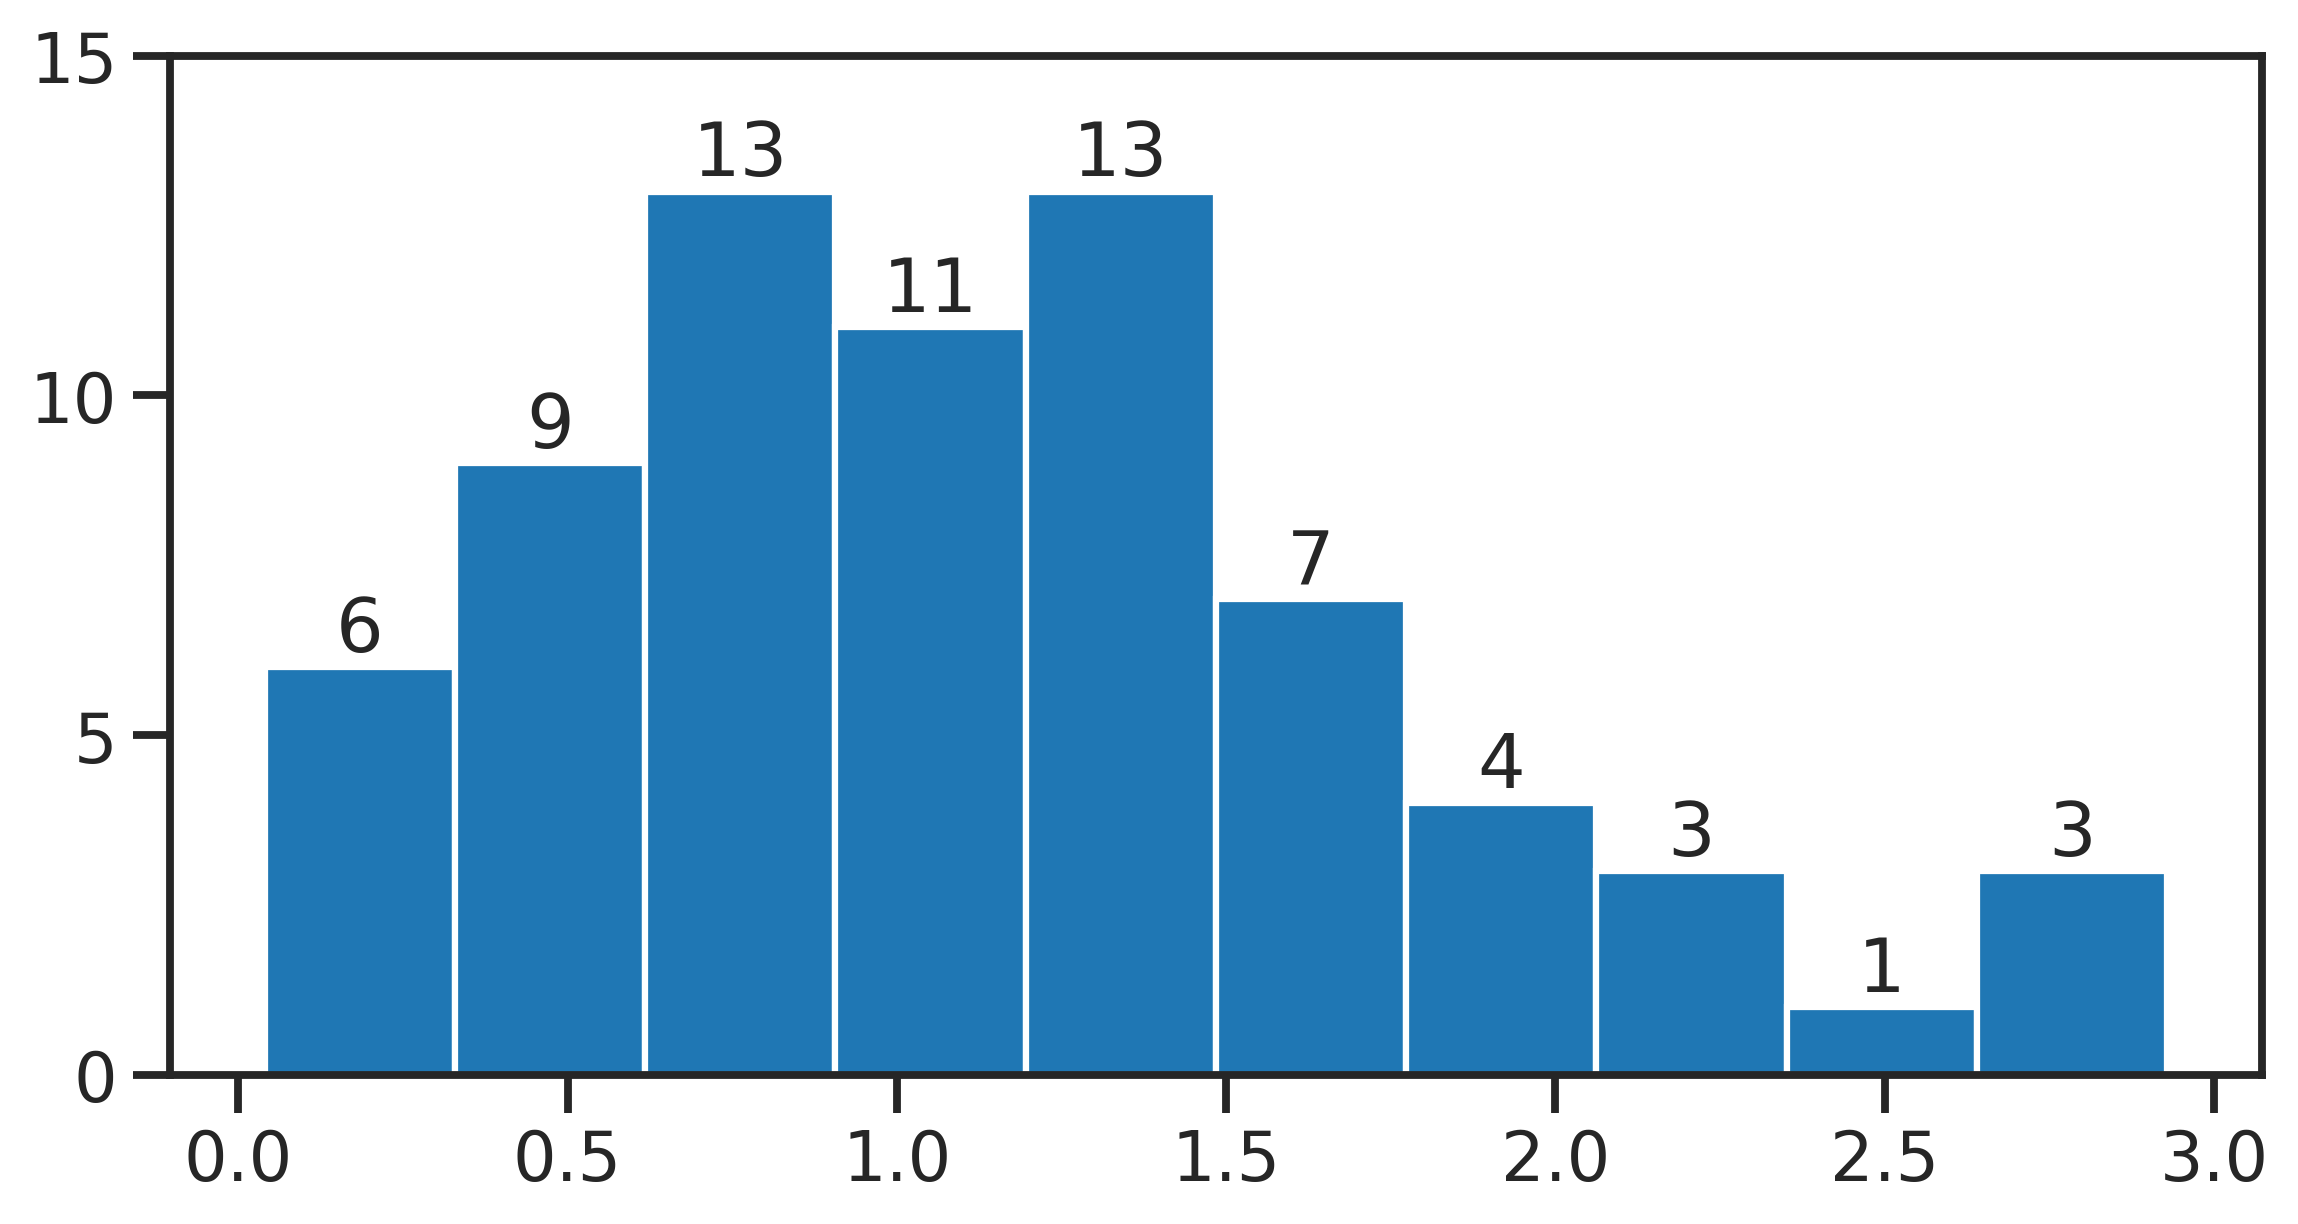
\includegraphics[width=0.8\textwidth]{./../pic/bar_example.png}
 	
 	\дз{Напишите в тетради формальное математическое описание bar-а.}
 	
\end{frame}



\begin{frame}{Перецентили, квантили}
	
	Параметр перцентиля $p$ -- это число от 0 до 100
	
	Перцентиль $percentile(V;p)$ -- это такое число, что $p\%$ элементов совокупности его не больше 
	и $(100-p)\%$ его элементов не меньше
	
	\дз{Напишите в тетради формальное математическое описание перцентиля}
	
	Квантиль -- это перцентиль заданный в диапазоне $0.0$ до $1.0$, а не в процентах.
	
	Можно переопределить медиану. 
	\begin{equation}
		median(V) = percentile(V;50)
	\end{equation}
\end{frame}


\begin{frame}{Дисперсия}

	
	Нужно ввести величину показывающую насколько выборка отходит от среднего значения. Если это число равно 0 -- то все значения падают в центр, 
	если не сильно больше 0 -- то около центра, если много больше -- то сильно 
	
	Введём центрированая совокупность $V_{center} = \{ v_{*}\} = \{v - median(V)\}$.
	
	Её значения могут быть как положительными, так и отрицательными, поэтому нужно либо брать $ \lVert v_* \rVert$ либо $v_*^2$ для анализа.
	
	Так как количество элементов различно -- разумно брать среднее от этих величин.
	
	Исторически сложилось брать квадрат, а не модуль.
	
	...
	
\end{frame}

\begin{frame}{Дисперсия}
	...
	Таким образом на языке математики:
	
	\begin{equation}
	variance(V) = mean(\{v_{*}^2\}) = \frac{\sum_{\forall v \in V} (v-mean(V))^2}{\lVert V \rVert}
	\end{equation}
	
	\дз{Прочитайте про моменты случайной величины. Что такое коэффициент асимметрии? Что такое коэффициент эксцесса?}
	
\end{frame}

\begin{frame}{Статистический выброс}
	Статистический выброс -- это значения, <<выделяющееся из общей выборки>> $V$.
	
	\begin{block}{Замечание}
	Выбор границы <<выделяющиесности>> -- отдельное инженерное искусство...
	Обычно всё анализируют через дисперсию (и другие моменты). 
	Но это детский сад. Реальные данные -- сложнее!
	\end{block}

	Часто выбросы выкидывают из анализа и анализируют повторно.

\end{frame}

\section{Ковариация, корреляция. Неравенсткво Коши-Буняковского}\label{section:correlation}

\begin{frame}{Ковариация}
	Пусть даны две совокупности: 
	$V_1 = \{v_1^1, v_2^1, ..., v_n^1\}$ и
    $V_2 = \{v_1^2, v_2^2, ..., v_n^2\}$,
	являющиеся 1-м и 2-м аргументами сложной совокупности 
	$V = \{(v_1^1, v_1^2), (v_2^1, v_2^2), ... (v_n^1, v_n^2)\}$. 
	
	Ковариация -- это математическое ожидание произведений $v_i^1 \cdot v_i^2$ минус произведение математических ожиданий $v_i^1$ и $v_i^2$.
	
	\begin{equation}\label{eq:cov_def}
	cov(V_1, V_2) = mean(\left\{\forall (v^1_i, v^2_i) \in V: v^1_i \cdot v^2_i\right\}) - mean(V_1) \cdot mean(V_2)
	\end{equation}

	\дз{Посмотрите как определяется ковариация в учебнике. Выведите формулу \eqref{eq:cov_def}.}
\end{frame}

\begin{frame}{Ковариация}
	
	Если $cov(V_1, V_2)=0$ -- величины независимы.
	
	\begin{block}{Замечание}
		К сожалению ковариация и МАТЕМАТИЧЕСКАЯ независимость / зависимость не всегда соотносится с реальным миром.
		(см. пример про маргарин и разводы из второй лекции).
		
		Поэтому всегда если можно другими способами проверить информацию -- лучше сделать это.
		
		С другой стороны можно по аналогии с <<утиным принципом>> в программировании аналогично рассуждать и по поводу ковариации.
		<<Если что-то выглядит как утка, плавает как утка и крякает как утка -- то это утка.>>
	\end{block}
\end{frame}

\begin{frame}{Неравенство Коши-Буняковского}
	
	Без доказательства:
	\begin{equation}
	cov^2 (V_1, V_2) \leqslant variance(V_1) \cdot variance(V_2) 
	\end{equation}
	
	\внекурса{После окончания DSIS-а найдите 2-3 понятных доказательства неравенства.}
	
\end{frame}


\begin{frame}{Линейный коэффициент корреляции}
	
	
	Линейный коэффициент корреляции, или коэффициент корреляции Пирсона, а чаще просто
	<<корреляция>> -- это величина:
	
	\begin{equation}
	cor (V_1, V_2) = \frac{cov(V_1, V_2)}{\sqrt{variance(V_1) \cdot variance(V_2)}} 
	\end{equation}
	
	Из неравенства Коши-Буняковского следует:
	\begin{equation}
	-1 \leqslant cor (V_1, V_2) \leqslant 1
	\end{equation}
	
	
\end{frame}


%\section{Манипуляции в статистике: математика.}

%\begin{frame}{Квартет Энскомба}
	
%\end{frame}

%\section{Манипуляции в статистике: общество.}
  
%\section{Манипуляции в статистике: ИБ.}


\end{document}